\documentclass[10pt,a4paper]{article}
\usepackage[utf8]{inputenc}
\usepackage[brazil]{babel}
\usepackage{graphicx}
\usepackage{amssymb, amsfonts, amsmath}
\usepackage{color}
\usepackage{float}
\usepackage{enumerate}
%\usepackage{subfigure}
\usepackage[top=2.5cm, bottom=2.5cm, left=1.25cm, right=1.25cm]{geometry}

\newcommand{\sen}{\,\textrm{sen}\,}
\newcommand{\tg}{\,\textrm{tg}\,}

\begin{document}
\pagestyle{empty}

\begin{center}
\begin{tabular}{ccc}
\begin{tabular}{c}

\includegraphics[scale=0.25]{../../biblioteca/imagem/brasao-de-armas-brasil} \\
\end{tabular} & 
\begin{tabular}{c}
Ministério da Educação \\
Universidade Federal dos Vales do Jequitinhonha e Mucuri \\
Faculdade de Ciências Sociais, Aplicadas e Exatas - FACSAE \\
Departamento de Ciências Exatas - DCEX \\
Disciplina: Cálculo Numérico\\
Prof.: Luiz C. M. de Aquino\\
\end{tabular} &
\begin{tabular}{c}

\includegraphics[scale=0.25]{../../biblioteca/imagem/logo-ufvjm} \\
\end{tabular}
\end{tabular}
\end{center}

\begin{center}
 \textbf{Lista de Exercícios XI}
\end{center}

\begin{enumerate}
  
  \item Considere o seguinte Problema de Valor Inicial (PVI):
  $$\begin{cases}
      y' = x^2y^2 \\
      y(-1) = \dfrac{6}{7}
    \end{cases}.
  $$
  \begin{enumerate}
    \item Aplique o Método de Euler para aproximar a solução deste PVI no intervalo $[-1;\, 1]$ considerando que ele foi dividido em $10$ 
          partes iguais.
    \item Verifique que a solução deste PVI é dada por $y(x) = \dfrac{-6}{2x^3 - 5}$. Faça o esboço do gráfico de $y$ no intervalo $[-1,\, 1]$ 
          juntamente com a solução aproximada obtida no item $(a)$.
  \end{enumerate}

   \item Considere o seguinte PVI:
  $$\begin{cases}
      y'' - xy' = 4 \\
      y(2) = 1 \\
      y'(2) = 5
    \end{cases}.
  $$
  
  Arrume este problema de modo que ele se transforme em um sistema com duas equações de primeira ordem. Em seguida, utilize o Método de Euler 
 para calcular a sua solução aproximada no intervalo $[2;\, 3]$, considerando uma subdivisão deste intervalo em $10$ partes iguais.

\end{enumerate}

\begin{center}
\textbf{Gabarito}
\end{center} 
\textbf{[1]} (a)
\begin{tabular}{c|c}
$x_k$ & $y_k$ \\ \hline
-1,0 & 0,85714285714285 \\ \hline
-0,8 & 1,00408163265306 \\ \hline
-0,6 & 1,13312866305706 \\ \hline
-0,4 & 1,22557526388405 \\  \hline
-0,2 & 1,27364037516227 \\ \hline
0,0 & 1,28661765360422 \\ \hline
0,2 & 1,28661765360422 \\ \hline
0,4 & 1,29986073349675 \\ \hline
0,6 & 1,35392914714432 \\ \hline
0,8 & 1,48591408489938 \\ \hline
1,0 & 1,76853049036528
\end{tabular} 
(b) %\begin{figure}[H]
      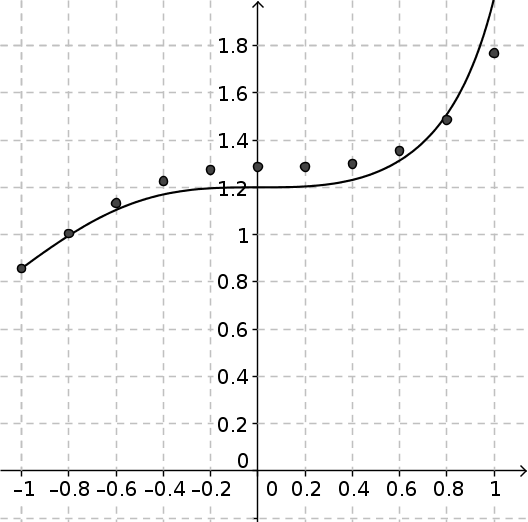
\includegraphics[scale=1]{imagem/figura1_listaxi.png}
     %\end{figure} 
\textbf{[2]} Definindo $y' = u$, podemos montar o sistema $\begin{cases}y' = u \\ u' = xu + 4 \\ y(2) = 1 \\ u(2) = 5\end{cases}$. Aplicando o Método de Euler, obtemos a tabela a seguir: 
\begin{tabular}{c|c|c}
$x_k$ & $u_k$ & $y_k$ \\ \hline
2,0 & 5,0 & 1,0  \\ \hline
2,1 & 6,4 & 1,5 \\ \hline
2,2 & 8,144 & 2,14 \\ \hline
2,3 & 10,33568 & 2,9544 \\ \hline
2,4 & 13,1128864 & 3,987968 \\ \hline
2,5 & 16,659979136 & 5,29925664 \\ \hline
2,6 & 21,22497392 & 6,9652545536 \\ \hline
2,7 & 27,1434671392 & 9,0877519456 \\ \hline
2,8 & 34,872203266784 & 11,80209865952 \\ \hline
2,9 & 45,0364201814836 & 15,2893189861984 \\ \hline
3,0 & 58,4969820341138 & 19,7929610043468
\end{tabular}.
\end{document}
